\documentclass{article}

\usepackage{graphicx}
\usepackage{tikz}
\usepackage{tikzsymbols}
\usetikzlibrary{calc,patterns,shapes.geometric}
\pagestyle{empty}
\usepackage[margin=0pt]{geometry}
\geometry{papersize={14in,12in}}

\def\centerarc[#1](#2)(#3:#4:#5){\draw[#1] ($(#2)+({#5*cos(#3)},{#5*sin(#3)})$) arc (#3:#4:#5);}

\begin{document}
	\begin{figure}
		\centering
		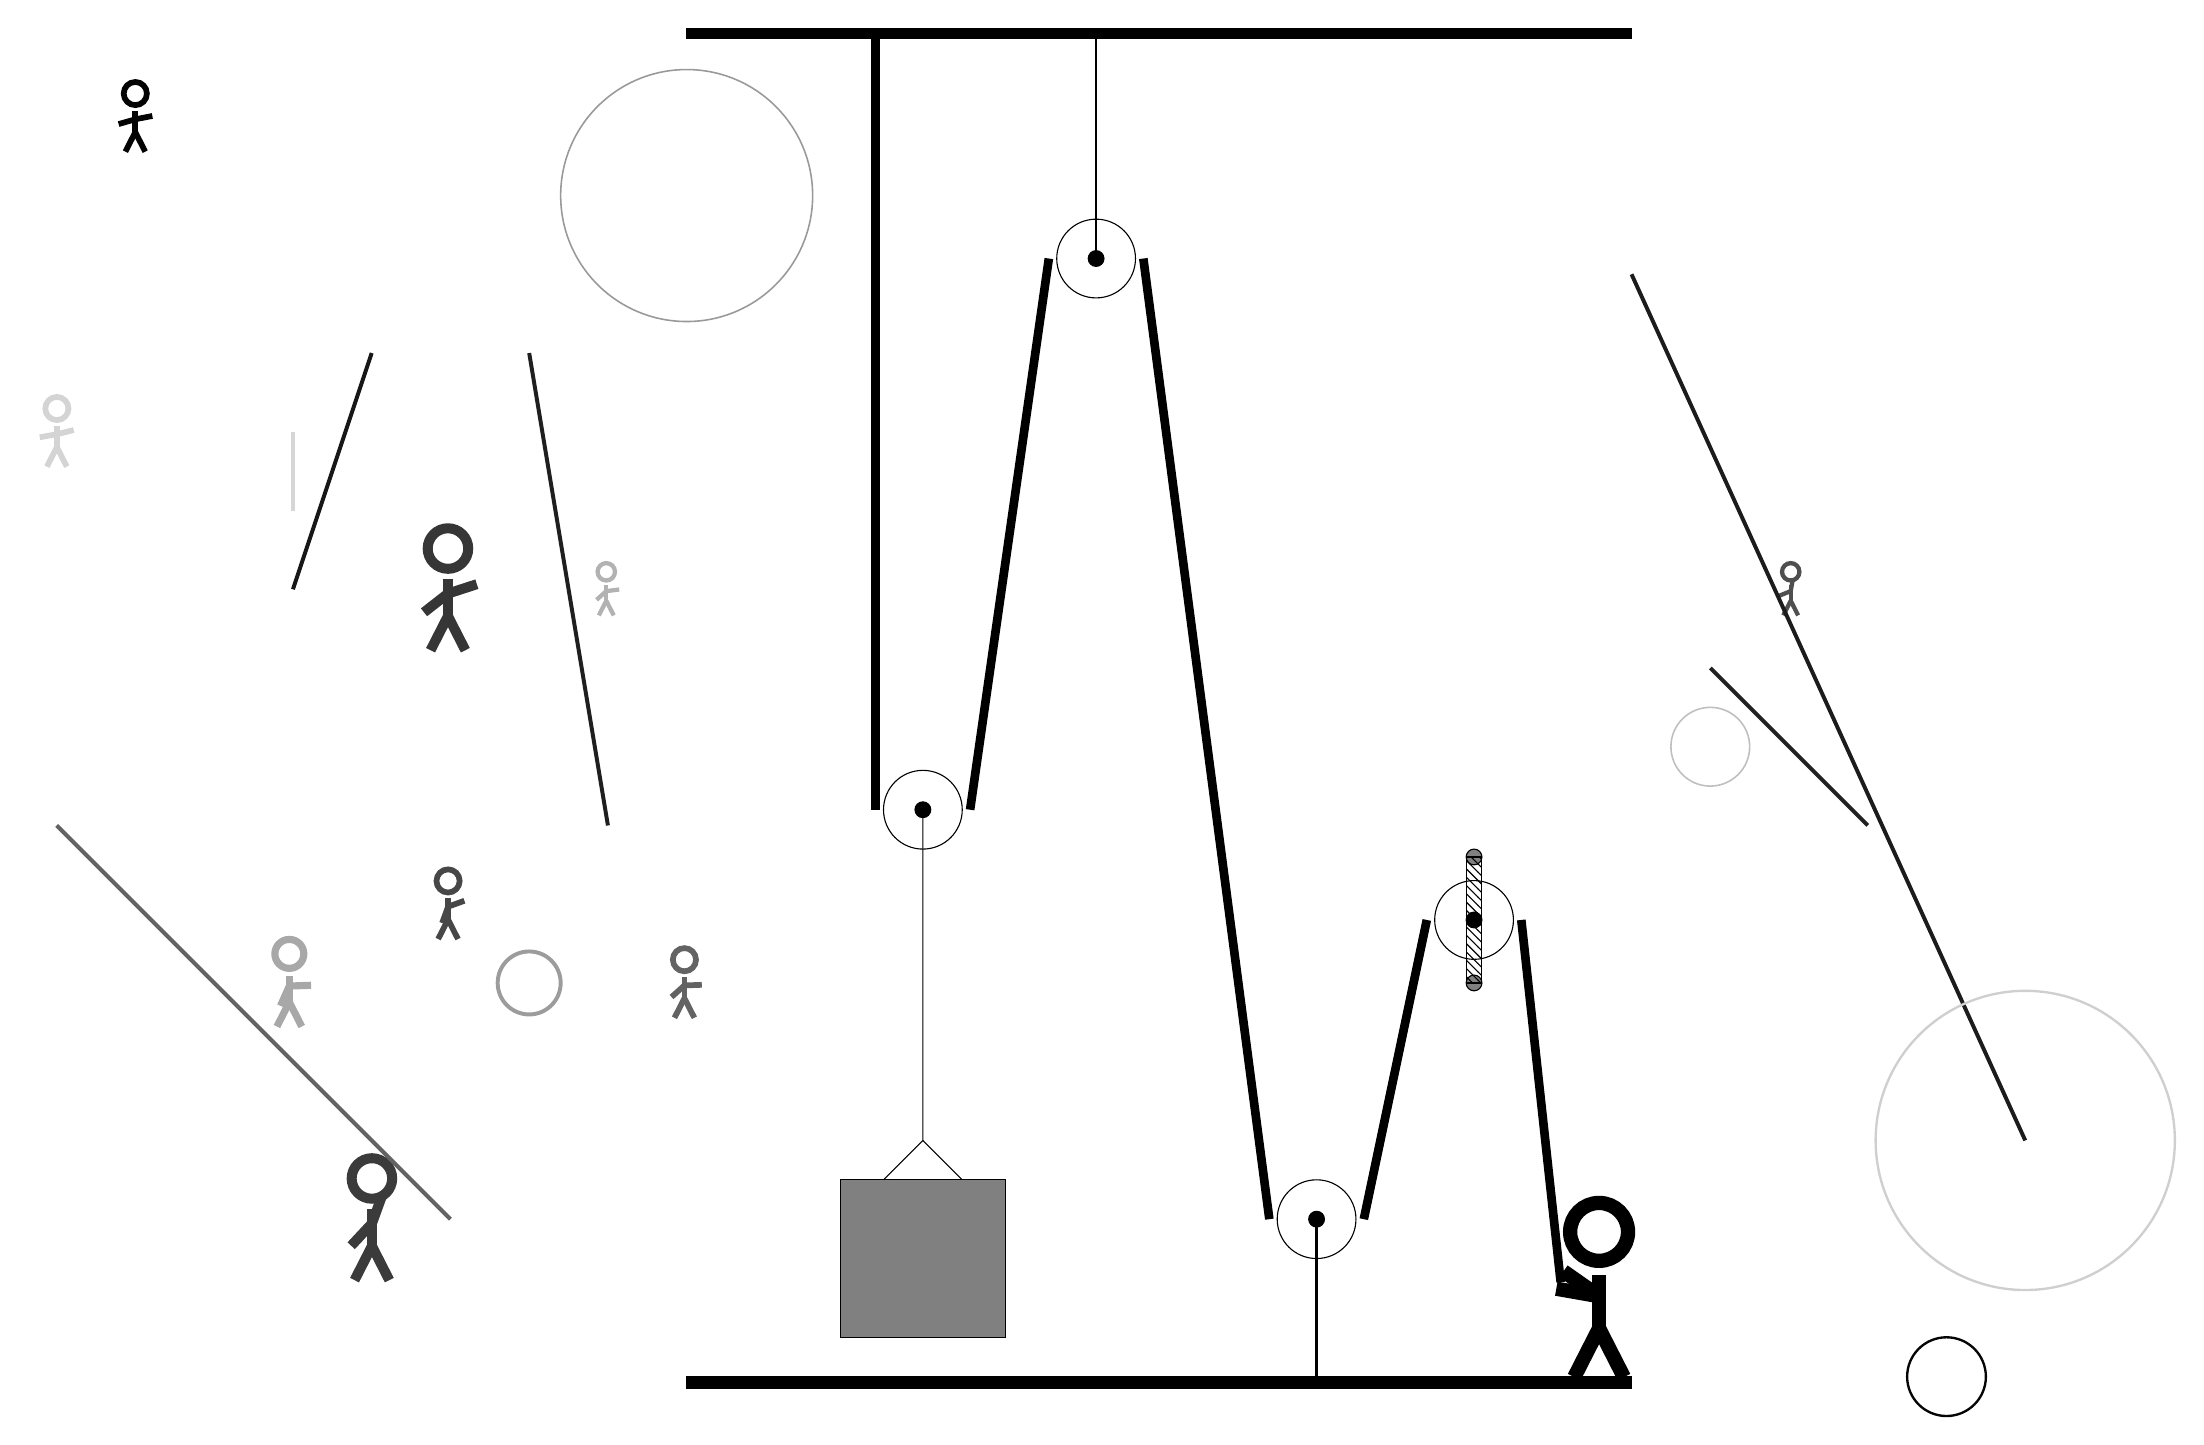
\begin{tikzpicture}
			%%%%% START %%%%%
			
			\draw[fill=black] (-2, 14) rectangle (10, 14.125);
			
			\draw (1, 4.2) circle (0.5);
			\draw[fill=black] (1, 4.2) circle (0.1);
			
			\draw (3.2, 11.2) circle (0.5);
			\draw[fill=black] (3.2, 11.2) circle (0.1);
			\draw[thick] (3.2, 11.2) -- (3.2, 14);
			
			\draw (6, -1) circle (0.5);
			\draw[fill=black] (6, -1) circle (0.1);
			\draw[thick] (6, -1) -- (6, -3);
			
			\draw [line width=0.3mm, color=black!98](14, -3) circle (0.5);
			
			\draw [line width=0.2mm, color=black!40](-2, 12) circle (1.6);
			\node[line width=0.2mm, color=black!30] at (-3, 7) {\Strichmaxerl[3][42][7]};
			\node[line width=0.6mm, color=black!69] at (12, 7) {\Strichmaxerl[3][22][80]};
			\draw [line width=0.5mm, color=black!39](-4, 2) circle (0.4);
			
			\node[line width=0.3mm, color=black!34] at (-7, 2) {\Strichmaxerl[5][66][2]};
			\node[line width=0.7mm, color=black!99] at (-9, 13) {\Strichmaxerl[4][16][11]};
			\draw[line width=0.5mm, color=black!89](10, 11) -- (15, 0);
			\node[line width=0.2mm, color=black!17] at (-10, 9) {\Strichmaxerl[4][10][14]};
			\node[line width=0.5mm, color=black!72] at (-5, 3) {\Strichmaxerl[4][70][20]};
			
			\draw[line width=0.5mm, color=black!87](11, 6) -- (13, 4);
			\draw[line width=0.5mm, color=black!91](-7, 7) -- (-6, 10);
			\draw[line width=0.5mm, color=black!88](-3, 4) -- (-4, 10);
			
			\node[line width=0.5mm, color=black!61] at (-2, 2) {\Strichmaxerl[4][42][2]};
			\node[line width=0.3mm, color=black!77] at (-6, -1) {\Strichmaxerl[7][47][70]};
			\draw [line width=0.3mm, color=black!19](15, 0) circle (1.9);
			\draw[line width=0.5mm, color=black!16](-7, 9) -- (-7, 8);
			
			\draw [line width=0.2mm, color=black!25](11, 5) circle (0.5);
			\draw[line width=0.5mm, color=black!61](-5, -1) -- (-10, 4);
			\node[line width=0.4mm, color=black!79] at (-5, 7) {\Strichmaxerl[7][38][18]};
			
			\draw[fill=white](8, 2.8) circle (0.5);
			\draw[fill=black] (8, 2.8) circle (0.1);
			\draw[fill=black!50] (8, 3.6) circle (0.1);
			\draw[fill=black!50] (8, 2.0) circle (0.1);
			\draw[pattern=north west lines, pattern color=black] (7.9, 3.6) rectangle (8.1, 2.0);
			
			\draw (1, 4.2) -- (1, 0) -- (0.5, -0.5);
			\draw (1, 0) -- (1.5, -0.5);
			\draw[fill=black!50] (-0.05, -0.5) rectangle (2.05, -2.5);
			
			\draw[line width=1.1mm] (0.4, 14) -- (0.4, 4.2);
			\centerarc[line width=1.1mm](1, 4.2)(180:360:0.6);
			\draw[line width=1.1mm](1.6, 4.2) -- (2.6, 11.2);
			\centerarc[line width=1.1mm](3.2, 11.2)(0:180:0.6);
			\draw[line width=1.1mm](3.8, 11.2) -- (5.4, -1);
			\centerarc[line width=1.1mm](6, -1)(180:360:0.6);
			\draw[line width=1.1mm](6.6, -1) -- (7.4, 2.8);
			\centerarc[line width=1.1mm](8, 2.8)(0:180:0.6);
			\draw[line width=1.1mm](8.6, 2.8) -- (9.1, -1.8);
			
			\node at (9.5, -1.9) {\Strichmaxerl[10][-35][170]};
			
			\draw[fill=black] (-2, -3) rectangle (10, -3.15);
			
			%%%%% END %%%%%
		\end{tikzpicture}
	\end{figure}	
\end{document}